% !TEX root = trabajo_final_arinc429.tex
\documentclass[12pt,a4paper,oneside]{report}

\usepackage[utf8]{inputenc}
\usepackage[T1]{fontenc}
\usepackage[spanish,es-tabla]{babel}
\usepackage[a4paper,margin=2.5cm]{geometry}
\usepackage{graphicx}
\usepackage{float}
\usepackage{booktabs}
\usepackage{longtable}
\usepackage{array}
\usepackage{xcolor}
\usepackage{tikz}
\usepackage{caption}
\usepackage{subcaption}
\usepackage{hyperref}
\usepackage{enumitem}
\usepackage{listings}
\usepackage{amsmath}
\usepackage{amssymb}

\usetikzlibrary{babel,arrows.meta,positioning,shapes.geometric,fit,calc}

\graphicspath{
  {../../imagenes/validacion_2026-06-19/}
  {../../imagenes/validacion_2026-06-29/}
  {../../imagenes/FWD/CH1 - CH2/}
  {../../imagenes/REV/CH1 - CH2/}
}

\hypersetup{
  colorlinks=true,
  linkcolor=blue!45!black,
  urlcolor=blue!45!black,
  citecolor=blue!45!black,
  pdftitle={Diseno e implementacion de un sniffer ARINC 429 logico},
  pdfauthor={Matias Diaz Benini}
}

\definecolor{pampaBlue}{RGB}{24,81,135}
\definecolor{pampaGreen}{RGB}{23,126,82}
\definecolor{pampaOrange}{RGB}{181,104,20}
\definecolor{pampaGray}{RGB}{80,88,96}
\definecolor{pampaLightBlue}{RGB}{235,244,252}
\definecolor{pampaLightGreen}{RGB}{236,248,241}
\definecolor{pampaLightOrange}{RGB}{255,246,232}

\lstset{
  basicstyle=\ttfamily\small,
  breaklines=true,
  frame=single,
  columns=fullflexible,
  keepspaces=true
}

\newcommand{\titulo}{Diseno e implementacion de un sniffer ARINC 429 logico con captura pasiva, transporte SPI y visualizacion web}
\newcommand{\autor}{Matias Diaz Benini}
\newcommand{\director}{[Completar]}
\newcommand{\institucion}{[Completar institucion]}
\newcommand{\carrera}{[Completar carrera]}
\newcommand{\fechaentrega}{Junio de 2026}

\newcommand{\metric}[2]{\textbf{#1} & #2 \\}

\begin{document}

\begin{titlepage}
  \centering
  \vspace*{1.5cm}
  {\Large \institucion\par}
  \vspace{0.4cm}
  {\large \carrera\par}
  \vspace{2.0cm}
  {\Huge\bfseries \titulo\par}
  \vspace{2.0cm}
  {\Large Trabajo Final de Grado\par}
  \vspace{1.5cm}
  \begin{tabular}{rl}
    Autor: & \autor \\
    Tutor / Director: & \director \\
    Fecha: & \fechaentrega \\
  \end{tabular}
  \vfill
  {\large Proyecto PAMPA / ARINC 429\par}
\end{titlepage}

\pagenumbering{roman}

\chapter*{Dedicatoria}
\addcontentsline{toc}{chapter}{Dedicatoria}

A quienes acompanaron el desarrollo del trabajo, sostuvieron las pruebas de
laboratorio y aportaron criterio tecnico para convertir una idea experimental
en un sistema medible, repetible y documentado.

\chapter*{Agradecimientos}
\addcontentsline{toc}{chapter}{Agradecimientos}

Se agradece al tutor del proyecto por las observaciones tecnicas realizadas
durante el desarrollo, especialmente las referidas a integridad de datos,
transporte por tramas completas, errores operativos en cero, mediciones de
osciloscopio y robustez ante fallas. Tambien se agradece la disponibilidad de
instrumental, placas y espacio de laboratorio que permitieron validar el
sistema durante corridas prolongadas.

\chapter*{Hoja de aceptacion}
\addcontentsline{toc}{chapter}{Hoja de aceptacion}

\vspace{1cm}
\begin{center}
\begin{tabular}{p{0.28\textwidth}p{0.55\textwidth}}
  Titulo del trabajo: & \titulo \\
  Autor: & \autor \\
  Tutor / Director: & \director \\
  Institucion: & \institucion \\
  Carrera: & \carrera \\
  Fecha: & \fechaentrega \\
\end{tabular}
\end{center}

\vspace{2.5cm}
\begin{center}
\begin{tabular}{p{0.38\textwidth}p{0.38\textwidth}}
  \hrulefill & \hrulefill \\
  Firma del tutor & Firma del evaluador \\
  \\[1.2cm]
  \hrulefill & \hrulefill \\
  Firma del evaluador & Firma del evaluador \\
\end{tabular}
\end{center}

\tableofcontents
\listoffigures
\listoftables

\chapter*{Glosario y convenciones}
\addcontentsline{toc}{chapter}{Glosario y convenciones}

\begin{longtable}{p{0.22\textwidth}p{0.70\textwidth}}
\toprule
\textbf{Termino} & \textbf{Descripcion} \\
\midrule
ARINC 429 & Bus aeronautico simplex basado en palabras de 32 bits y senalizacion bipolar con retorno a cero. \\
FWD & Canal directo observado en el laboratorio, desde la placa transmisora hacia la receptora. \\
REV & Canal inverso disponible como segundo canal observable por el sniffer. \\
RZ & Return to Zero. Cada bit vuelve a nivel nulo durante parte de su celda temporal. \\
Label & Campo de 8 bits que identifica el significado de una palabra ARINC. \\
SDI & Source/Destination Identifier. Campo usado como subidentificador de fuente o destino. \\
SSM & Sign/Status Matrix. Campo usado para estado o signo de la palabra. \\
PIO & Programmable I/O de Raspberry Pi Pico, usado para temporizacion deterministica. \\
SPI & Serial Peripheral Interface, usado entre el sniffer y la Raspberry Pi 3B+. \\
DRDY & Data Ready. Linea digital que indica a la 3B+ que hay un snapshot disponible. \\
Bridge & Servicio Python en la 3B+ que traduce SPI a HTTP/JSON y metricas. \\
Supervisor & Servicio de vigilancia que controla bridge y dashboard, y clasifica el estado del sistema. \\
\bottomrule
\end{longtable}

\chapter*{Resumen}
\addcontentsline{toc}{chapter}{Resumen}

El trabajo desarrolla una plataforma de laboratorio para generar, recibir,
capturar y visualizar trafico compatible a nivel logico y temporal con ARINC
429. La solucion implementa un transmisor, un receptor, un sniffer pasivo, un
bridge SPI/HTTP en Raspberry Pi 3B+ y un dashboard web con metricas para
Prometheus y Grafana. El transmisor genera palabras de 32 bits con codificacion
bipolar logica con retorno a cero, operando a 100 kbps o 12.5 kbps. El sniffer
observa el canal sin intervenirlo, filtra por label y SDI, verifica paridad,
detecta automaticamente la velocidad del enlace y entrega snapshots al host por
SPI en tramas completas de 32 bytes. La Raspberry Pi 3B+ publica los datos por
HTTP y supervisa los servicios mediante un proceso independiente. La validacion
incluyo mediciones de osciloscopio, prueba de paridad estricta, barrido de
frecuencia SPI, recuperacion ante fallas y dos corridas finales de ocho horas.
Los ensayos finales cerraron con cero errores SPI operativos, cero errores de
paridad, cero overflow, cero drops SPI y deteccion estable de 100 kbps y 12.5
kbps. El resultado es un sistema reproducible, observable y documentado para
analisis de trafico ARINC 429 en condiciones controladas de laboratorio.

\chapter*{Palabras claves}
\addcontentsline{toc}{chapter}{Palabras claves}

ARINC 429; Raspberry Pi Pico; PIO; SPI; sniffer pasivo; Flask; Prometheus;
Grafana; retorno a cero; avionica; adquisicion de datos.

\pagenumbering{arabic}

\chapter{Introduccion}

ARINC 429 es una arquitectura de comunicacion ampliamente difundida en sistemas
aeronauticos. Su interes tecnico surge de combinar una palabra de datos fija,
un canal simplex, una temporizacion estricta y una codificacion fisica con
retorno a cero. Estas caracteristicas permiten estudiar problemas de
temporizacion, integridad, captura pasiva y observabilidad de datos en tiempo
real.

El presente trabajo implementa una plataforma experimental que reproduce el
comportamiento logico y temporal de un enlace ARINC 429 mediante placas
Raspberry Pi Pico y una Raspberry Pi 3B+. El sistema no se limita a transmitir
datos: incorpora un sniffer pasivo, un transporte robusto hacia host, un
dashboard operativo, metricas historicas y procedimientos de validacion. La
motivacion principal es disponer de una herramienta controlada y repetible para
analizar trafico ARINC 429, verificar palabras, medir temporizacion y demostrar
robustez de captura durante corridas prolongadas.

El alcance del trabajo se define sobre senales logicas de 3.3 V generadas en
laboratorio. Dentro de ese alcance se implemento la palabra ARINC, la
codificacion bipolar logica con retorno a cero, la transmision a 100 kbps y
12.5 kbps, la captura pasiva, la deteccion automatica de velocidad, el rechazo
por paridad, el transporte SPI por tramas completas, la visualizacion web y la
observabilidad por Prometheus/Grafana.

\section{Problema abordado}

La captura de un enlace tipo ARINC exige resolver simultaneamente varios
aspectos:

\begin{itemize}
  \item generar una temporizacion estable e independiente de la carga de CPU;
  \item reconstruir palabras de 32 bits a partir de dos lineas logicas;
  \item capturar el enlace sin modificar la comunicacion observada;
  \item transportar datos hacia un host sin perder integridad;
  \item distinguir errores de arranque de errores operativos reales;
  \item registrar evidencias objetivas de funcionamiento.
\end{itemize}

El sistema construido resuelve estos puntos mediante PIO en las Pico,
transporte SPI por trama completa, linea DRDY, supervisor de servicios y
registro estadistico automatizado.

\section{Alcance}

El alcance tecnico validado incluye:

\begin{itemize}
  \item transmision FWD sobre dos GPIO en modo bipolar logico;
  \item recepcion de palabras FWD por una segunda Pico;
  \item sniffer pasivo sobre FWD y REV;
  \item labels de telemetria: temperatura, velocidad y altitud;
  \item filtro por label y SDI;
  \item paridad impar de palabra ARINC;
  \item deteccion autonoma de 100 kbps y 12.5 kbps;
  \item enlace SPI a 8 MHz entre sniffer y 3B+;
  \item dashboard Flask y metricas Prometheus;
  \item corridas finales de ocho horas.
\end{itemize}

\chapter{Objetivos}

\section{Objetivo general}

Disenar, implementar y validar una plataforma de laboratorio capaz de generar,
recibir, capturar y visualizar trafico ARINC 429 logico, con sniffer pasivo,
transporte SPI robusto y observabilidad web.

\section{Objetivos especificos}

\begin{enumerate}
  \item Implementar un transmisor capaz de emitir palabras ARINC de 32 bits con
  retorno a cero a 100 kbps y 12.5 kbps.
  \item Implementar un receptor que reconstruya palabras a partir del par
  logico FWD y verifique integridad.
  \item Implementar un sniffer pasivo que observe FWD y REV sin transmitir
  sobre el enlace ARINC.
  \item Filtrar palabras por label y SDI, y rechazar palabras con paridad
  incorrecta.
  \item Transportar snapshots y estadisticas hacia una Raspberry Pi 3B+ por
  SPI en tramas completas.
  \item Publicar datos operativos mediante HTTP/JSON, dashboard Flask y
  metricas Prometheus.
  \item Registrar evidencias en CSV, JSON y PDF.
  \item Validar estabilidad mediante osciloscopio y corridas prolongadas.
\end{enumerate}

\section{Destinatarios}

El trabajo esta destinado a docentes, evaluadores y estudiantes de electronica,
telecomunicaciones, sistemas embebidos y avionica que requieran una plataforma
practica para estudiar comunicacion ARINC 429 a nivel logico y temporal.

\section{Beneficios}

Los beneficios principales son:

\begin{itemize}
  \item plataforma reproducible para ensayos de comunicacion avionica;
  \item separacion clara entre generacion, recepcion, sniffing y visualizacion;
  \item instrumentacion directa con osciloscopio;
  \item trazabilidad de resultados por JSON, CSV y PDF;
  \item comparacion entre 100 kbps y 12.5 kbps;
  \item validacion de integridad con errores operativos en cero;
  \item bajo costo de implementacion al usar placas de desarrollo disponibles.
\end{itemize}

\chapter{Estudio tecnico}

\section{Modelo ARINC 429 utilizado}

ARINC 429 define una comunicacion simplex: un transmisor emite palabras hacia
uno o mas receptores. En el modelo implementado se trabaja con dos lineas
logicas por canal, denominadas A y B. Para representar la senal bipolar:

\begin{itemize}
  \item bit logico alto: A bajo, B alto en la representacion de la PIO usada;
  \item bit logico bajo: A alto, B bajo;
  \item nivel nulo: A bajo y B bajo.
\end{itemize}

La observacion diferencial mediante osciloscopio, en modo MATH, permite ver
valores aproximados de +3.3 V, 0 V y -3.3 V. En el laboratorio esta amplitud es
logica y no corresponde a una interfaz electrica certificada de campo.

\section{Formato de palabra}

Cada palabra transporta 32 bits. La implementacion organiza la informacion en
label, SDI, dato, SSM y paridad impar.

\begin{table}[H]
\centering
\caption{Campos principales de la palabra ARINC implementada}
\begin{tabular}{lll}
\toprule
Campo & Bits & Uso en el sistema \\
\midrule
Label & 1--8 & Identificador de variable \\
SDI & 9--10 & Subidentificador de fuente/destino \\
Dato & 11--29 & Magnitud codificada \\
SSM & 30--31 & Estado de la palabra \\
Paridad & 32 & Paridad impar \\
\bottomrule
\end{tabular}
\end{table}

\section{Labels utilizados}

\begin{table}[H]
\centering
\caption{Labels utiles de la plataforma}
\begin{tabular}{llll}
\toprule
Label & SDI & Nombre & Unidad \\
\midrule
0xA5 & 0 & TEMPERATURA & C \\
0xB1 & 1 & VELOCIDAD & kt \\
0xC2 & 2 & ALTITUD & ft \\
0xAC & 3 & ACK\_BATCH & batch \\
\bottomrule
\end{tabular}
\end{table}

La operacion final utiliza principalmente temperatura, velocidad y altitud. El
label ACK\_BATCH queda contemplado en el protocolo y en el filtro para observar
trafico inverso cuando exista actividad por REV.

\section{Codificacion bipolar logica con retorno a cero}

Cada bit se divide en dos mitades:

\begin{itemize}
  \item primera mitad: nivel activo, positivo o negativo;
  \item segunda mitad: retorno a nivel nulo.
\end{itemize}

A 100 kbps el bit dura 10 us: 5 us activos y 5 us nulos. A 12.5 kbps el bit
dura 80 us: 40 us activos y 40 us nulos.

\begin{figure}[H]
\centering
\begin{tikzpicture}[x=0.85cm,y=0.8cm,>=Latex]
  \draw[->] (0,0) -- (12.5,0) node[right]{tiempo};
  \draw[->] (0,-1.6) -- (0,1.8) node[above]{nivel diferencial};
  \draw[dashed,gray] (0,1) -- (12,1);
  \draw[dashed,gray] (0,-1) -- (12,-1);
  \node[left] at (0,1) {$+V$};
  \node[left] at (0,-1) {$-V$};
  \node[left] at (0,0) {$0$};
  \draw[very thick,pampaBlue]
    (0,0) -- (0,1) -- (1,1) -- (1,0) -- (2,0)
    -- (2,-1) -- (3,-1) -- (3,0) -- (4,0)
    -- (4,1) -- (5,1) -- (5,0) -- (6,0)
    -- (6,1) -- (7,1) -- (7,0) -- (8,0)
    -- (8,-1) -- (9,-1) -- (9,0) -- (10,0)
    -- (10,-1) -- (11,-1) -- (11,0) -- (12,0);
  \foreach \x in {0,2,4,6,8,10,12} {
    \draw[gray!70] (\x,-1.35) -- (\x,1.45);
  }
  \draw[<->] (0,-1.35) -- (2,-1.35) node[midway,below]{1 bit};
  \node at (1,1.35){1};
  \node at (3,-1.35){0};
  \node at (5,1.35){1};
  \node at (7,1.35){1};
  \node at (9,-1.35){0};
  \node at (11,-1.35){0};
\end{tikzpicture}
\caption{Representacion conceptual de la codificacion bipolar logica con retorno a cero.}
\end{figure}

\section{Seleccion tecnologica}

La seleccion se baso en disponibilidad, temporizacion deterministica y
capacidad de observacion.

\begin{longtable}{p{0.24\textwidth}p{0.32\textwidth}p{0.34\textwidth}}
\caption{Tecnologias seleccionadas}\\
\toprule
Elemento & Tecnologia & Fundamento \\
\midrule
\endfirsthead
\toprule
Elemento & Tecnologia & Fundamento \\
\midrule
\endhead
Transmision y recepcion & Raspberry Pi Pico / PIO & Permite temporizacion por hardware sin depender del lazo principal de CPU. \\
Sniffer & Raspberry Pi Pico / PIO & Permite observar dos canales y ejecutar SPI slave por trama completa. \\
Host & Raspberry Pi 3B+ & Dispone de Linux, SPI, Ethernet, Python y servicios HTTP. \\
Visualizacion & Flask & Dashboard liviano para operacion directa. \\
Historico & Prometheus/Grafana & Scraping y visualizacion temporal de metricas. \\
Transporte sniffer-host & SPI a 8 MHz & Margen suficiente para snapshots sin limitar el enlace ARINC. \\
Arranque de servicios & systemd & Autoarranque, reinicio automatico y trazabilidad por logs. \\
\bottomrule
\end{longtable}

\section{Alternativas analizadas}

\subsection{UART, I2C y SPI}

UART fue descartado como transporte principal entre sniffer y host por su menor
capacidad para transacciones estructuradas con reloj controlado por el host.
I2C ofrece direccionamiento simple, pero no resulta conveniente para rafagas de
telemetria y snapshots a alta tasa. SPI permite que la Raspberry Pi 3B+ actue
como master, controle el reloj y lea estructuras completas de 32 bytes con bajo
overhead.

\subsection{SPI byte a byte y SPI por trama}

El modo byte a byte fue util como base estable. La implementacion final usa
tramas completas de 32 bytes en PIO porque responde mejor al requisito de
transportar paquetes atomicos, reduce ambiguedades de sincronizacion y permite
un protocolo mas auditable.

\subsection{Polling y DRDY}

El polling periodico funciona, pero realiza consultas aun cuando no hay datos
nuevos. El modo DRDY usa una linea adicional: el sniffer sube GP20 cuando hay
snapshot nuevo y la 3B+ consulta por SPI. El sistema conserva timeout como
respaldo si se pierde una transicion.

\subsection{Wi-Fi y Ethernet directo}

La configuracion recomendada usa Ethernet directo entre notebook y 3B+. Esta
red reduce jitter operativo y mantiene separada la comunicacion local del
trafico Wi-Fi.

\chapter{Arquitectura del sistema}

\section{Vista general}

\begin{figure}[H]
\centering
\resizebox{\textwidth}{!}{%
\begin{tikzpicture}[
  block/.style={draw,rounded corners,minimum width=3.0cm,minimum height=1.25cm,align=center,thick,fill=pampaLightBlue},
  bus/.style={draw,rounded corners,minimum width=5.1cm,minimum height=1.0cm,align=center,thick,fill=pampaLightGreen},
  host/.style={draw,rounded corners,minimum width=3.2cm,minimum height=1.25cm,align=center,thick,fill=pampaLightOrange},
  arrow/.style={-Latex,thick}
]
  \node[block] (tx) {ARINC-TX\\Pico\\GP2/GP3};
  \node[bus,right=2.2cm of tx] (fwd) {Canal FWD\\par logico A/B\\100 kbps o 12.5 kbps};
  \node[block,right=2.2cm of fwd] (rx) {ARINC-RX\\Pico\\entrada FWD};
  \node[block,below=1.8cm of fwd] (snf) {ARINC-SNIFFER\\Pico\\tap pasivo FWD/REV};
  \node[host,below=1.8cm of snf] (pi) {Raspberry Pi 3B+\\Bridge HTTP/SPI\\Flask};
  \node[host,right=2.4cm of pi] (nb) {Notebook\\Prometheus\\Grafana\\Navegador};

  \draw[arrow] (tx) -- (fwd);
  \draw[arrow] (fwd) -- (rx);
  \draw[arrow,pampaGreen] (fwd) -- node[right,align=center]{conexion\\pasiva} (snf);
  \draw[arrow,pampaOrange] (snf) -- node[right]{SPI + DRDY} (pi);
  \draw[arrow] (pi) -- node[above]{Ethernet} (nb);
\end{tikzpicture}}
\caption{Arquitectura general del sistema implementado. El sniffer se conecta al cable observado, no a una placa como emisor.}
\end{figure}

\section{Distribucion fisica}

\begin{table}[H]
\centering
\caption{Placas y responsabilidades}
\begin{tabular}{p{0.22\textwidth}p{0.68\textwidth}}
\toprule
Placa & Funcion \\
\midrule
ARINC-TX & Genera palabras utiles y ruido controlado, selecciona velocidad y transmite FWD. \\
ARINC-RX & Recibe FWD, reconstruye palabras, valida paridad y procesa stream. \\
ARINC-SNIFFER & Observa FWD y REV, filtra, valida paridad, mantiene snapshots y responde por SPI. \\
Raspberry Pi 3B+ & Ejecuta bridge, dashboard Flask, recorder y supervisor. \\
Notebook & Visualiza dashboard, Prometheus y Grafana por Ethernet. \\
\bottomrule
\end{tabular}
\end{table}

\section{Red y servicios}

\begin{figure}[H]
\centering
\begin{tikzpicture}[
  svc/.style={draw,rounded corners,align=center,minimum width=3.6cm,minimum height=1.0cm,fill=pampaLightBlue,thick},
  arrow/.style={-Latex,thick}
]
  \node[svc] (bridge) {Bridge\\127.0.0.1:5100};
  \node[svc,right=2.0cm of bridge] (flask) {Flask\\0.0.0.0:5000};
  \node[svc,right=2.0cm of flask] (prom) {Prometheus\\127.0.0.1:9090};
  \node[svc,below=1.2cm of prom] (graf) {Grafana\\127.0.0.1:3000};
  \node[svc,below=1.2cm of bridge] (sup) {Supervisor\\systemd};

  \draw[arrow] (bridge) -- node[above]{HTTP loopback} (flask);
  \draw[arrow] (flask) -- node[above]{/metrics} (prom);
  \draw[arrow] (prom) -- (graf);
  \draw[arrow] (sup) -- node[left]{GET /stats} (bridge);
  \draw[arrow] (sup) -- node[below]{systemctl status} (flask);
\end{tikzpicture}
\caption{Servicios en host y observabilidad. El bridge no se expone a la red externa.}
\end{figure}

\chapter{Desarrollo del hardware logico}

\section{ARINC-TX}

La placa transmisora genera una secuencia de palabras de telemetria. El target
principal es:

\begin{lstlisting}
arinc_tx_arinc429_logic_stream_autorate
\end{lstlisting}

Este firmware selecciona al arrancar una de dos velocidades:

\begin{itemize}
  \item 100000 bps;
  \item 12500 bps.
\end{itemize}

La seleccion se realiza en firmware mediante una semilla basada en tiempo de
arranque. Para ensayos controlados existe tambien el target
\texttt{arinc\_tx\_arinc429\_logic\_stream\_12k5}, que fuerza 12.5 kbps.

\begin{figure}[H]
\centering
\resizebox{0.95\textwidth}{!}{%
\begin{tikzpicture}[
  b/.style={draw,rounded corners,align=center,minimum width=2.6cm,minimum height=1.1cm,fill=pampaLightBlue,thick},
  arrow/.style={-Latex,thick}
]
  \node[b] (rng) {Seleccion\\100k / 12.5k};
  \node[b,right=1.2cm of rng] (data) {Generador\\temperatura\\velocidad\\altitud};
  \node[b,right=1.2cm of data] (word) {Encoder\\label + SDI\\dato + SSM};
  \node[b,right=1.2cm of word] (par) {Paridad\\impar};
  \node[b,right=1.2cm of par] (pio) {PIO TX\\RZ bipolar\\FWD};
  \draw[arrow] (rng) -- (data);
  \draw[arrow] (data) -- (word);
  \draw[arrow] (word) -- (par);
  \draw[arrow] (par) -- (pio);
\end{tikzpicture}}
\caption{Flujo interno del transmisor.}
\end{figure}

La PIO recibe la palabra por FIFO, desplaza 32 bits y genera dos salidas. Para
cada bit emite una mitad activa y luego un nivel nulo. La temporizacion se
define por divisor de clock, por lo que el tiempo de bit no depende del tiempo
de ejecucion del lazo principal.

\section{ARINC-RX}

La placa receptora observa el par FWD. Su state machine PIO espera actividad en
cualquiera de los hilos, clasifica el simbolo segun el pin activo, espera el
retorno a nulo y reconstruye 32 bits. El target final es:

\begin{lstlisting}
arinc_rx_arinc429_logic_stream
\end{lstlisting}

El receptor no necesita que el transmisor le informe la velocidad. El criterio
de recepcion se basa en actividad y retorno a nulo, no en una espera fija de
10 us. Por eso puede reconstruir palabras tanto a 100 kbps como a 12.5 kbps,
siempre que la forma RZ sea respetada.

\begin{figure}[H]
\centering
\resizebox{0.95\textwidth}{!}{%
\begin{tikzpicture}[
  b/.style={draw,rounded corners,align=center,minimum width=2.8cm,minimum height=1.0cm,fill=pampaLightGreen,thick},
  arrow/.style={-Latex,thick}
]
  \node[b] (pins) {Entrada\\FWD A/B};
  \node[b,right=1.2cm of pins] (pio) {PIO RX\\espera activo\\espera nulo};
  \node[b,right=1.2cm of pio] (fifo) {FIFO RX\\palabra 32 bits};
  \node[b,right=1.2cm of fifo] (cpu) {CPU\\paridad\\label/SDI};
  \node[b,right=1.2cm of cpu] (stats) {Stats\\y log USB};
  \draw[arrow] (pins) -- (pio);
  \draw[arrow] (pio) -- (fifo);
  \draw[arrow] (fifo) -- (cpu);
  \draw[arrow] (cpu) -- (stats);
\end{tikzpicture}}
\caption{Flujo interno del receptor.}
\end{figure}

\section{ARINC-SNIFFER}

El sniffer es el nucleo del trabajo. Observa FWD y REV sin transmitir sobre
esas lineas. La comunicacion activa del sniffer ocurre exclusivamente hacia la
Raspberry Pi 3B+ por SPI.

El target usado es:

\begin{lstlisting}
sniffer_arinc429_logic_pio_frame
\end{lstlisting}

La build validada informa:

\begin{lstlisting}
SPI-PIOFRAME-ARINC429-STRICTPARITY-DRDY-AUTORATE-RECOVERY-V5
\end{lstlisting}

\begin{figure}[H]
\centering
\resizebox{\textwidth}{!}{%
\begin{tikzpicture}[
  b/.style={draw,rounded corners,align=center,minimum width=2.8cm,minimum height=1.0cm,fill=pampaLightOrange,thick},
  c/.style={draw,rounded corners,align=center,minimum width=2.8cm,minimum height=1.0cm,fill=pampaLightBlue,thick},
  arrow/.style={-Latex,thick}
]
  \node[b] (in) {FWD/REV\\tap pasivo};
  \node[b,right=1.0cm of in] (pio) {PIO RX\\2 canales};
  \node[b,right=1.0cm of pio] (class) {CPU\\palabra\\paridad\\label/SDI};
  \node[b,right=1.0cm of class] (snap) {Snapshot\\16 slots};
  \node[c,below=1.2cm of snap] (spi) {PIO SPI slave\\trama 32 bytes};
  \node[c,left=1.0cm of spi] (drdy) {DRDY\\GP20};
  \draw[arrow] (in) -- (pio);
  \draw[arrow] (pio) -- (class);
  \draw[arrow] (class) -- (snap);
  \draw[arrow] (snap) -- (spi);
  \draw[arrow] (snap) -- (drdy);
\end{tikzpicture}}
\caption{Flujo interno del sniffer.}
\end{figure}

\subsection{Filtro e integridad}

El sniffer usa una whitelist de hasta 10 entradas. En la configuracion de
validacion:

\begin{lstlisting}
0xA5/0
0xB1/1
0xC2/2
0xAC/3
\end{lstlisting}

Una palabra se acepta si:

\begin{enumerate}
  \item coincide con label y SDI permitidos;
  \item cumple la paridad impar;
  \item su magnitud es plausible para la variable decodificada;
  \item corresponde al canal esperado cuando se trata de ACK.
\end{enumerate}

Las palabras con paridad incorrecta incrementan el contador de error, pero no
actualizan el snapshot ni \texttt{accepted\_words}.

\subsection{Deteccion automatica de velocidad}

El sniffer calcula una tasa de palabras FWD dentro de una ventana de 2 s. Si la
tasa supera el umbral alto, clasifica el enlace como 100 kbps. Si supera el
umbral bajo pero no el alto, lo clasifica como 12.5 kbps. El resultado se
publica como:

\begin{lstlisting}
detected_bit_rate_bps
detected_bit_rate_txt
\end{lstlisting}

En SPI se transporta en el payload de meta como
\texttt{detected\_bit\_rate\_hz\_div100}. La 3B+ lo multiplica por 100 para
reconstruir la velocidad en bps.

\subsection{Recuperacion de captura}

Ante una resincronizacion, la state machine se detiene, limpia FIFO, reinicia
su estado interno y espera un intervalo de canal nulo antes de volver a
capturar. El tiempo de reposo requerido cambia segun la velocidad detectada.
Esto evita reengancharse en medio de una palabra.

\chapter{Transporte SPI y software host}

\section{Protocolo SPI}

El protocolo SPI usa paquetes de 32 bytes. Cada paquete contiene magic,
version, comando, estado, secuencia, payload y CRC16.

\begin{table}[H]
\centering
\caption{Estructura del paquete SPI}
\begin{tabular}{lll}
\toprule
Campo & Tamano & Descripcion \\
\midrule
Magic & 2 bytes & 0xA4, 0x29 \\
Version & 1 byte & Version de protocolo \\
Command & 1 byte & Comando solicitado \\
Status & 1 byte & Estado de respuesta \\
Flags & 1 byte & Flags auxiliares \\
Sequence & 2 bytes & Secuencia \\
Payload & 22 bytes & Datos del comando \\
CRC16 & 2 bytes & Integridad del paquete \\
\bottomrule
\end{tabular}
\end{table}

Comandos principales:

\begin{table}[H]
\centering
\caption{Comandos SPI utilizados}
\begin{tabular}{lll}
\toprule
Comando & Codigo & Funcion \\
\midrule
PING & 0x01 & Verifica enlace SPI \\
GET\_STATS & 0x03 & Lee contadores globales \\
GET\_FILTER & 0x04 & Lee filtro activo \\
SET\_FILTER & 0x05 & Configura filtro \\
RESET\_STATS & 0x06 & Reinicia contadores \\
GET\_LATEST\_META & 0x07 & Lee metadata de snapshot \\
GET\_LATEST\_SLOT & 0x08 & Lee un slot de snapshot \\
\bottomrule
\end{tabular}
\end{table}

\section{SPI por PIO-frame}

El slave SPI del sniffer se implementa en PIO. La state machine RX espera CS
activo, lee 8 palabras de 32 bits y completa una trama de 32 bytes. La state
machine TX entrega la respuesta sincronizada con SCK. Esta implementacion evita
depender del SPI slave hardware de la Pico y permite controlar el armado de
paquetes completos.

\section{DRDY}

La linea DRDY conecta:

\begin{lstlisting}
Pico GP20 -> Raspberry Pi GPIO25
\end{lstlisting}

Cuando el snapshot cambia, el sniffer sube DRDY. La 3B+ detecta el nivel y
solicita metadata y slots por SPI. Si no se detecta DRDY, el bridge conserva un
timeout periodico para mantener el estado actualizado.

\section{Bridge HTTP/SPI}

El bridge corre en la 3B+ y queda ligado a loopback:

\begin{lstlisting}
http://127.0.0.1:5100
\end{lstlisting}

Sus responsabilidades son:

\begin{itemize}
  \item inicializar SPI;
  \item manejar CS manual;
  \item leer DRDY;
  \item consultar snapshots;
  \item decodificar payloads;
  \item exponer \texttt{/stats}, \texttt{/metrics} y endpoints de control;
  \item separar errores de arranque de errores operativos.
\end{itemize}

Configuracion validada:

\begin{lstlisting}
ARINC_SPI_HZ=8000000
ARINC_SPI_TRANSFER_MODE=pio-frame
ARINC_SPI_REQUEST_MODE=drdy
ARINC_SPI_MANUAL_CS=1
ARINC_SPI_CS_GPIO=8
ARINC_SPI_CS_SETUP_US=100
ARINC_SPI_CS_HOLD_US=100
ARINC_SPI_DRDY_GPIO=25
ARINC_SPI_DRDY_TIMEOUT_SEC=0.250
\end{lstlisting}

\section{Dashboard Flask}

Flask consulta al bridge local y publica una vista operativa en:

\begin{lstlisting}
http://192.168.50.2:5000
\end{lstlisting}

La interfaz muestra:

\begin{itemize}
  \item palabras aceptadas;
  \item paridad OK y errores de paridad;
  \item errores SPI;
  \item bitrate detectado;
  \item estado del supervisor;
  \item ultimas variables: temperatura, velocidad y altitud;
  \item distribucion por label y SSM.
\end{itemize}

\section{Prometheus y Grafana}

Flask expone \texttt{/metrics}. Prometheus scrapea esas metricas desde la
notebook y Grafana permite visualizacion historica. La vista Flask se usa para
operacion rapida; Prometheus/Grafana se usan para tendencia y diagnostico.

\section{Supervisor}

El supervisor corre como servicio systemd independiente. Consulta \texttt{/stats}
y el estado de servicios. Clasifica el sistema en estados como RUNNING,
WAITING\_SNIFFER, SPI\_SYNCING, CABLE\_FAULT, BRIDGE\_FAULT y RECOVERING.

Durante las corridas finales el supervisor permanecio en:

\begin{lstlisting}
supervisor_state = RUNNING
supervisor_health = ok
\end{lstlisting}

No ejecuto acciones correctivas durante las ocho horas de cada prueba final.

\chapter{Metodologia de desarrollo y validacion}

\section{Procedimiento general}

La metodologia combino desarrollo incremental, instrumentacion directa y
corridas prolongadas. Cada cambio relevante se valido primero con diagnosticos
cortos y luego con pruebas largas.

\begin{enumerate}
  \item Compilacion de firmware TX, RX y SNIFFER.
  \item Carga de UF2 en cada Pico.
  \item Verificacion de conexion SPI con diagnostico 12/12.
  \item Arranque de bridge, Flask y supervisor.
  \item Verificacion de \texttt{/stats}.
  \item Medicion instrumental con osciloscopio.
  \item Registro prolongado con \texttt{stats\_recorder.py}.
  \item Analisis de \texttt{summary.json}, \texttt{events.csv} y PDF generado.
\end{enumerate}

\section{Actividades realizadas}

\begin{longtable}{p{0.34\textwidth}p{0.18\textwidth}p{0.38\textwidth}}
\caption{Actividades principales del trabajo}\\
\toprule
Actividad & Duracion relativa & Resultado \\
\midrule
\endfirsthead
\toprule
Actividad & Duracion relativa & Resultado \\
\midrule
\endhead
Organizacion del repositorio & Media & Componentes separados por funcion. \\
Firmware TX/RX logico & Alta & Palabras ARINC logicas a 100 kbps y 12.5 kbps. \\
Sniffer pasivo & Alta & Captura FWD/REV, filtro, paridad y snapshots. \\
Transporte SPI & Alta & Paquetes de 32 bytes en PIO-frame. \\
Bridge y dashboard & Media & HTTP/JSON, Flask y metricas. \\
Supervisor & Media & Vigilancia y recuperacion automatica. \\
Osciloscopio & Media & Validacion de bit time, RZ y diferencial logico. \\
Corridas largas & Alta & Evidencia de estabilidad de 8 h por velocidad. \\
Documentacion & Alta & README, procedimientos, evidencias y reportes. \\
\bottomrule
\end{longtable}

\section{Instrumental y medios}

\begin{itemize}
  \item placas Raspberry Pi Pico / Pico 2 W;
  \item Raspberry Pi 3B+;
  \item notebook con Prometheus y Grafana;
  \item osciloscopio Tektronix;
  \item conexion Ethernet directa;
  \item cables dupont y conexion de masa comun;
  \item firmware en C con Pico SDK;
  \item scripts Python para bridge, recorder y supervisor.
\end{itemize}

\chapter{Resultados}

\section{Validacion con osciloscopio}

Las capturas de osciloscopio confirman:

\begin{itemize}
  \item amplitud logica individual aproximada de 3.3 V;
  \item retorno a cero en cada bit;
  \item bit time de 10 us a 100 kbps;
  \item bit time de 80 us a 12.5 kbps;
  \item lectura diferencial aproximada +3.3 V, 0 V y -3.3 V;
  \item palabras de 32 bits separadas por estado nulo.
\end{itemize}

\begin{figure}[H]
\centering
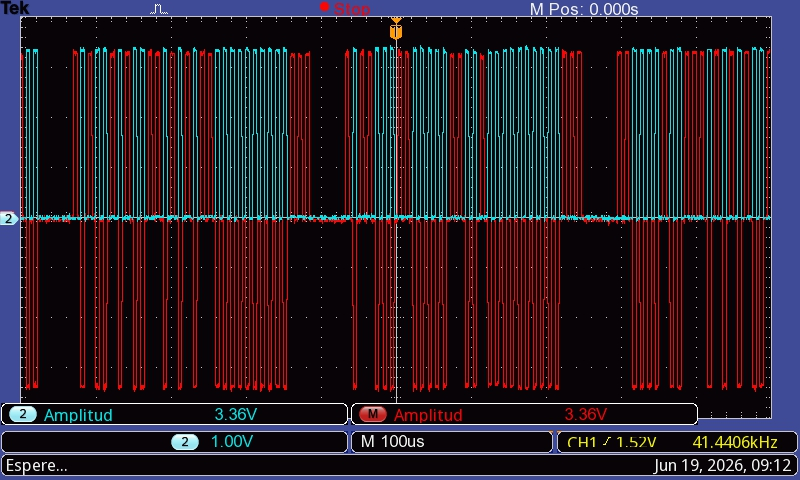
\includegraphics[width=0.92\textwidth]{TEK0007_MATH.JPG}
\caption{Captura MATH de senal diferencial logica. Se observan pulsos positivos, negativos y nivel nulo.}
\end{figure}

\begin{figure}[H]
\centering
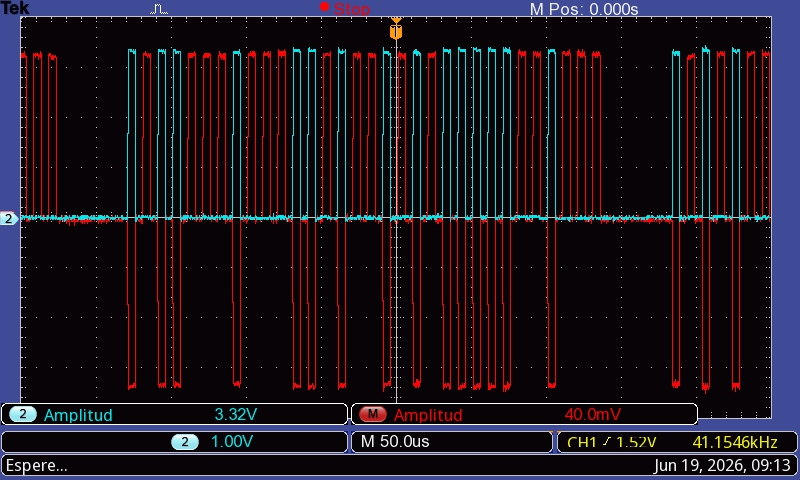
\includegraphics[width=0.92\textwidth]{TEK0008_MATH.JPG}
\caption{Secuencia de palabras sobre el canal observado con representacion diferencial.}
\end{figure}

\begin{figure}[H]
\centering
\begin{subfigure}{0.48\textwidth}
  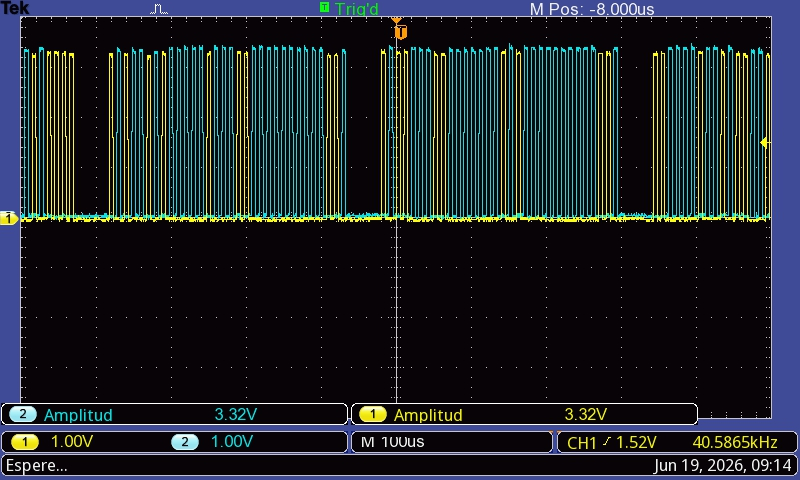
\includegraphics[width=\textwidth]{TEK0011_CANALES.JPG}
  \caption{Canales individuales A/B.}
\end{subfigure}
\hfill
\begin{subfigure}{0.48\textwidth}
  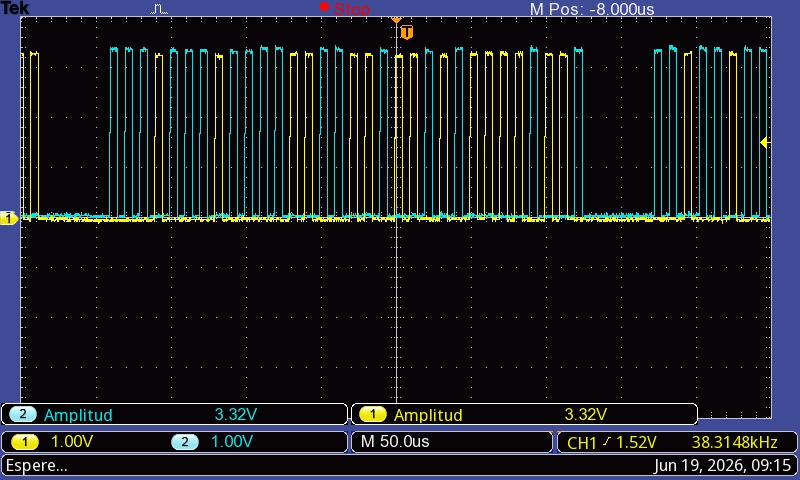
\includegraphics[width=\textwidth]{TEK0013_CANALES.JPG}
  \caption{Tren de pulsos sin MATH.}
\end{subfigure}
\caption{Medicion de canales logicos individuales. Los canales no se pisan: representan polaridades opuestas o estado nulo.}
\end{figure}

\subsection*{Validacion autorate final}

El 2026-06-29 se completo la evidencia instrumental de las dos velocidades del
modo autorate. Para 100 kbps se midio una palabra completa de 320 us, una
ventana palabra mas gap de 364 us y un gap visible de 44 us. Para 12.5 kbps se
midio una media celda activa de 40 us, un bit completo de 80 us y un gap visible
de 360 us.

\begin{table}[H]
\centering
\caption{Mediciones de osciloscopio para autorate}
\begin{tabular}{lll}
\toprule
Velocidad & Medicion & Valor \\
\midrule
100 kbps & Palabra completa & 320 us \\
100 kbps & Palabra + gap visible & 364 us \\
100 kbps & Gap visible & 44 us \\
12.5 kbps & Media celda activa & 40 us \\
12.5 kbps & Bit completo & 80 us \\
12.5 kbps & Palabra completa esperada & 2.56 ms \\
12.5 kbps & Gap visible & 360 us \\
\bottomrule
\end{tabular}
\end{table}

La relacion entre los gaps visibles medidos fue:

\begin{equation}
\frac{360\ \mu s}{44\ \mu s} = 8.18
\end{equation}

El resultado es consistente con la relacion teorica 8:1 entre 100 kbps y
12.5 kbps. La diferencia respecto del valor exacto se explica por la colocacion
manual de cursores y por medir el gap visible entre actividad de palabras en la
pantalla del osciloscopio.

\begin{figure}[H]
\centering
\begin{subfigure}{0.48\textwidth}
  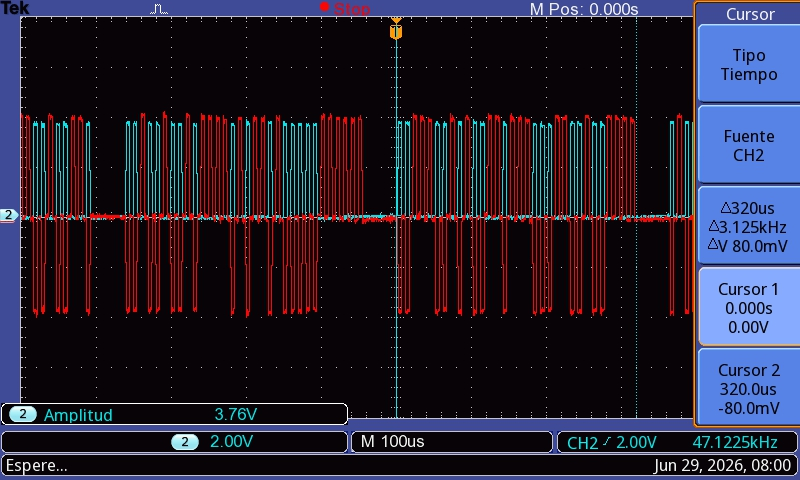
\includegraphics[width=\textwidth]{TEK0014_100k_palabra_320us.JPG}
  \caption{100 kbps: palabra de 320 us.}
\end{subfigure}
\hfill
\begin{subfigure}{0.48\textwidth}
  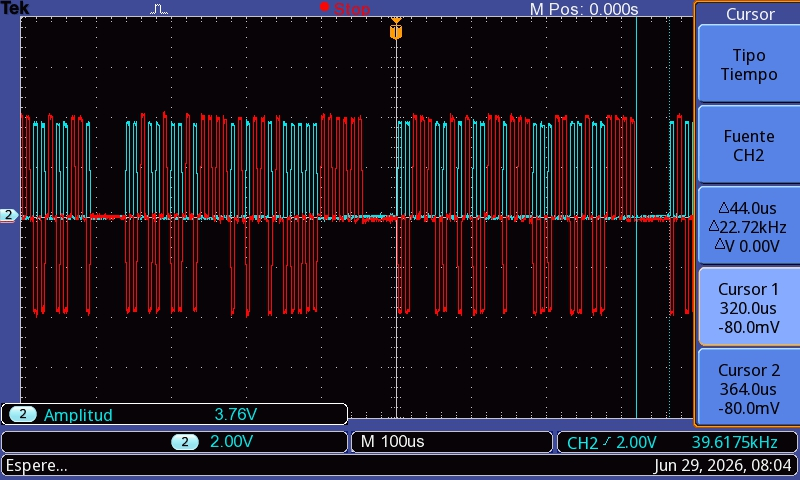
\includegraphics[width=\textwidth]{TEK0016_100k_gap_44us.JPG}
  \caption{100 kbps: gap visible de 44 us.}
\end{subfigure}
\caption{Mediciones temporales finales a 100 kbps.}
\end{figure}

\begin{figure}[H]
\centering
\begin{subfigure}{0.48\textwidth}
  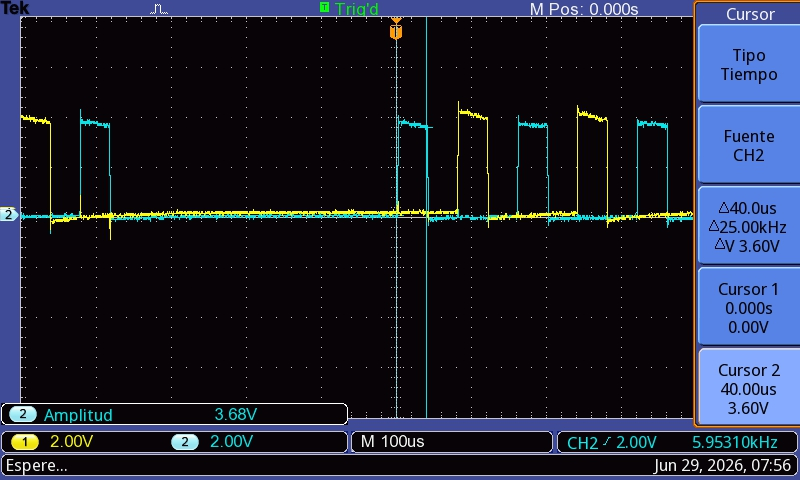
\includegraphics[width=\textwidth]{TEK0011_12k5_media_celda_40us.JPG}
  \caption{12.5 kbps: media celda activa de 40 us.}
\end{subfigure}
\hfill
\begin{subfigure}{0.48\textwidth}
  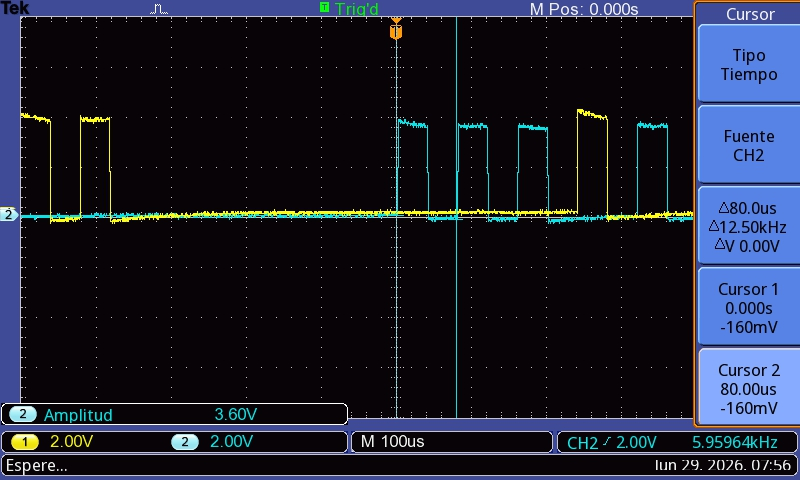
\includegraphics[width=\textwidth]{TEK0012_12k5_bit_80us.JPG}
  \caption{12.5 kbps: bit completo de 80 us.}
\end{subfigure}
\caption{Mediciones temporales finales a 12.5 kbps.}
\end{figure}

\begin{figure}[H]
\centering
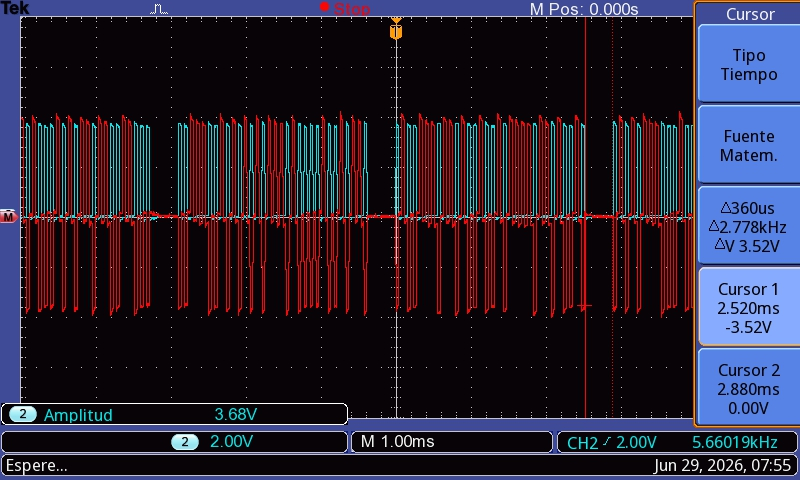
\includegraphics[width=0.86\textwidth]{TEK0009_12k5_gap_360us.JPG}
\caption{12.5 kbps: gap visible entre palabras de aproximadamente 360 us.}
\end{figure}

\section{Barrido de frecuencia SPI}

El barrido solicitado incluyo frecuencias hasta 50 MHz. La conclusion practica
fue seleccionar 8 MHz como perfil operativo con margen.

\begin{table}[H]
\centering
\caption{Resumen del barrido SPI}
\begin{tabular}{lll}
\toprule
Frecuencia & Resultado & Observacion \\
\midrule
100 kHz a 8 MHz & PASS & Respuestas validas \\
9 MHz & PASS & Valido en prueba corta \\
10 MHz & Parcial & 13/24 respuestas validas \\
16 MHz & FAIL & 0/24 \\
50 MHz & FAIL & Respuesta invalida / cero \\
\bottomrule
\end{tabular}
\end{table}

La frecuencia de SPI no necesita coincidir con la velocidad ARINC. ARINC es el
enlace observado; SPI es el transporte de telemetria ya decodificada entre
sniffer y host.

\section{Prueba de paridad estricta}

Se uso una variante con inyeccion deliberada de errores de paridad para validar
que el sniffer no entregue palabras corruptas a capas superiores.

\begin{table}[H]
\centering
\caption{Prueba de paridad estricta}
\begin{tabular}{lr}
\toprule
Metrica & Valor \\
\midrule
Palabras recibidas & 610905 \\
Errores de paridad detectados & 6109 \\
Balance de clasificacion & 0 \\
Errores SPI operativos & 0 \\
Resultado & PASS \\
\bottomrule
\end{tabular}
\end{table}

\section{Corridas finales autorate}

Las corridas finales validan las dos velocidades soportadas. Ambas duraron 8 h
con una muestra cada 5 s.

\begin{table}[H]
\centering
\caption{Comparacion de corridas finales}
\begin{tabular}{lrr}
\toprule
Metrica & 12.5 kbps & 100 kbps \\
\midrule
Sesion & \multicolumn{1}{c}{20260619\_212806} & \multicolumn{1}{c}{20260620\_065154} \\
Duracion [s] & 28801.451 & 28801.407 \\
Muestras & 5760 & 5760 \\
Velocidad detectada [bps] & 12500 & 100000 \\
Palabras recibidas & 9876638 & 76707606 \\
Palabras aceptadas & 2962992 & 23012283 \\
Palabras filtradas & 6913646 & 53695323 \\
Tasa media aceptada [words/s] & 102.876 & 798.999 \\
Tasa maxima aceptada [words/s] & 108.233 & 828.346 \\
Errores de paridad & 0 & 0 \\
Errores SPI operativos & 0 & 0 \\
Overflow & 0 & 0 \\
Drops SPI & 0 & 0 \\
Resync FWD operativos & 0 & 0 \\
Muestras desconectadas & 0 & 0 \\
Veredicto & PASS & PASS \\
\bottomrule
\end{tabular}
\end{table}

La relacion entre tasas medias aceptadas fue:

\begin{equation}
\frac{798.999}{102.876} = 7.77
\end{equation}

El valor es coherente con la relacion teorica 8:1 entre 100 kbps y 12.5 kbps.
La diferencia corresponde a rafagas, pausas aleatorias del generador y muestreo
discreto.

\section{Balance de contadores}

En ambas corridas se cumplio:

\begin{equation}
\text{received\_words} =
\text{accepted\_words} + \text{filtered\_words}
\end{equation}

Para 12.5 kbps:

\begin{equation}
9876638 = 2962992 + 6913646
\end{equation}

Para 100 kbps:

\begin{equation}
76707606 = 23012283 + 53695323
\end{equation}

Este cierre exacto muestra que la estadistica conserva todo el trafico
clasificado: lo recibido queda aceptado o filtrado, sin una tercera categoria
de perdida.

\section{Estado del supervisor}

Durante las corridas finales:

\begin{itemize}
  \item \texttt{supervisor\_state = RUNNING};
  \item \texttt{supervisor\_health = ok};
  \item \texttt{supervisor\_issue = none};
  \item acciones correctivas: 0;
  \item reinicios de servicio: 0;
  \item recuperaciones SPI: 0.
\end{itemize}

\chapter{Costos, operacion e impacto}

\section{Inversion requerida}

El prototipo se construyo con elementos de laboratorio y placas de desarrollo.
La inversion se organiza por rubros.

\begin{longtable}{p{0.32\textwidth}p{0.55\textwidth}}
\caption{Rubros de inversion}\\
\toprule
Rubro & Elementos \\
\midrule
\endfirsthead
\toprule
Rubro & Elementos \\
\midrule
\endhead
Recursos humanos & Desarrollo de firmware, scripts, dashboard, pruebas y documentacion. \\
Equipamiento & Raspberry Pi Pico, Raspberry Pi 3B+, notebook, osciloscopio, cables y fuente. \\
Software & Pico SDK, Python, Flask, Prometheus, Grafana y herramientas de compilacion. \\
Infraestructura & Mesa de laboratorio, red Ethernet directa y alimentacion USB. \\
Insumos & Cables, conectores, almacenamiento y soporte de montaje. \\
\bottomrule
\end{longtable}

El costo principal no estuvo en componentes electronicos, sino en horas de
ingenieria, pruebas y documentacion. El uso de hardware disponible redujo la
barrera de implementacion.

\section{Costos de operacion y mantenimiento}

Los costos de operacion son bajos:

\begin{itemize}
  \item consumo electrico reducido de placas y notebook;
  \item mantenimiento de scripts y firmware;
  \item reemplazo de cables o conectores si fallan;
  \item conservacion de evidencias y backups del repositorio.
\end{itemize}

\section{Viabilidad comercial}

El trabajo se plantea como plataforma tecnica de laboratorio. Su valor esta en
la capacidad de demostrar conceptos de comunicacion, captura pasiva y
observabilidad. No se formula aqui una comercializacion de producto; por lo
tanto el analisis economico se limita a la conveniencia tecnica y educativa del
prototipo construido.

\section{Impacto ambiental}

El impacto ambiental es bajo. El sistema usa placas de bajo consumo y no
requiere procesos contaminantes. La principal recomendacion operativa es
reutilizar hardware disponible, conservar cables y gestionar correctamente los
residuos electronicos al fin de su vida util.

\section{Impacto social y academico}

El aporte social y academico se concentra en:

\begin{itemize}
  \item formacion practica en sistemas embebidos;
  \item instrumentacion de protocolos avionicos;
  \item trazabilidad de pruebas;
  \item integracion entre electronica, software y redes;
  \item disponibilidad de una base reproducible para evaluacion docente.
\end{itemize}

\chapter{Dificultades y soluciones aplicadas}

\section{Errores SPI de arranque}

Al iniciar bridge y placas en momentos distintos, el host podia intentar leer
antes de que el sniffer estuviera listo. La solucion fue separar
\texttt{spi\_startup\_errors} de \texttt{spi\_errors}. Asi, los errores previos
a la primera comunicacion valida no contaminan la estadistica operativa.

\section{Transporte byte a byte}

El transporte inicial byte a byte era funcional, pero no expresaba una trama
atomica. Se implemento \texttt{pio-frame}, donde cada transaccion mueve un
paquete completo de 32 bytes.

\section{Polling}

El polling continuo generaba consultas innecesarias. Se agrego DRDY para que
el sniffer avise cuando hay snapshot nuevo. El sistema mantiene timeout como
respaldo.

\section{Reinicio o desconexion del sniffer}

El reinicio del sniffer podia dejar al bridge sincronizado con una respuesta
invalida. Se agrego reset de transporte por trama completa y recuperacion V5,
con espera de reposo del canal antes de reactivar captura.

\section{Gap temporal entre palabras}

Las mediciones iniciales mostraban separacion mayor a la esperada. El ajuste de
PIO TX dejo la celda de bit en 10 us a 100 kbps, con 5 us activos y retorno a
nulo, validado por osciloscopio. La validacion final registro tambien la
separacion visible entre palabras: 44 us a 100 kbps y 360 us a 12.5 kbps. La
relacion 360/44 = 8.18 confirma que la escala temporal del gap acompana el
cambio de velocidad esperado.

\section{Robustez de servicios}

Bridge y Flask se instalaron como servicios systemd con autoarranque. El
supervisor verifica estado y expone su condicion por \texttt{/stats} y
\texttt{/metrics}.

\chapter{Conclusiones}

El trabajo alcanzo el objetivo propuesto: se implemento y valido una plataforma
de laboratorio capaz de generar, recibir, sniffear y visualizar trafico ARINC
429 logico. La solucion integra hardware embebido, PIO, SPI, HTTP, dashboard,
metricas y registro estadistico.

Los resultados finales son consistentes y verificables. Las corridas de ocho
horas a 100 kbps y 12.5 kbps cerraron con cero errores SPI operativos, cero
errores de paridad, cero overflow, cero drops SPI, cero resync FWD operativos y
supervisor en estado sano. La tasa observada escala aproximadamente 8:1 entre
ambas velocidades, como predice la relacion teorica.

La medicion con osciloscopio confirmo el retorno a cero, la duracion de bit, la
forma diferencial logica, la palabra completa de 32 bits a 100 kbps y la escala
temporal correcta del modo 12.5 kbps. El transporte SPI por tramas completas, la
linea DRDY y el supervisor convierten al sistema en una plataforma operable y
no solo en una prueba aislada de firmware.

La arquitectura final queda ordenada por responsabilidades: TX genera trafico,
RX reconstruye palabras, SNIFFER observa pasivamente, la 3B+ traduce a HTTP y
la notebook registra y visualiza. Esta separacion facilita explicar el sistema,
repetir ensayos y auditar resultados.

\chapter{Referencias y bibliografia}

\begin{thebibliography}{9}

\bibitem{arinc429}
ARINC Specification 429.
\textit{Mark 33 Digital Information Transfer System}. Aeronautical Radio, Inc.

\bibitem{rp2040}
Raspberry Pi Ltd.
\textit{RP2040 Datasheet}. Programmable I/O, GPIO, DMA y perifericos.

\bibitem{pico-sdk}
Raspberry Pi Ltd.
\textit{Raspberry Pi Pico C/C++ SDK}.

\bibitem{flask}
Pallets Projects.
\textit{Flask Documentation}.

\bibitem{prometheus}
Prometheus Authors.
\textit{Prometheus Documentation}.

\bibitem{grafana}
Grafana Labs.
\textit{Grafana Documentation}.

\bibitem{repo}
Repositorio local del proyecto PAMPA / ARINC 429.
\textit{ARINC\_SPI}, rama \texttt{ARINC}, tag \texttt{arinc-logic-v1.1.0}.

\end{thebibliography}

\appendix

\chapter{Comandos operativos principales}

\section{Servicios en Raspberry Pi 3B+}

\begin{lstlisting}
systemctl status arinc-sniffer-bridge arinc-dashboard-flask arinc-supervisor --no-pager
curl http://127.0.0.1:5100/stats
curl http://127.0.0.1:5100/supervisor/status
\end{lstlisting}

\section{Prometheus y Grafana en notebook}

\begin{lstlisting}
cd "C:\Users\usuario\RASPI PICO\PAMPA\ARINC_SPI\prometheus"
powershell -ExecutionPolicy Bypass -File .\start_prometheus_grafana.ps1
\end{lstlisting}

\section{Registro estadistico}

\begin{lstlisting}
cd ~/PAMPA/HOST_3b+
source .venv/bin/activate
nohup python3 stats_recorder.py start \
  --name corrida_final_noche_autorate \
  --duration 28800 \
  --interval 5 \
  --tx-firmware arinc_tx_arinc429_logic_stream_autorate \
  --rx-firmware arinc_rx_arinc429_logic_stream \
  --sniffer-firmware sniffer_arinc429_logic_pio_frame \
  > stats_recorder.log 2>&1 &
\end{lstlisting}

\chapter{Archivos de evidencia}

\begin{itemize}
  \item \texttt{docs/evidencia\_corridas\_finales\_autorate\_8h.md}
  \item \texttt{docs/evidencia\_autorate\_100k\_12k5.md}
  \item \texttt{docs/evidencia\_osciloscopio\_arinc429\_20260619.md}
  \item \texttt{docs/evidencia\_barrido\_frecuencia\_spi.md}
  \item \texttt{docs/evidencia\_recuperacion\_fallas\_v5.md}
  \item \texttt{docs/entrega\_tutor/datos/summary\_corrida8h\_100k.json}
  \item \texttt{docs/entrega\_tutor/datos/summary\_corrida8h\_12k5.json}
  \item \texttt{docs/entrega\_tutor/reportes/reporte\_corrida8h\_100k.pdf}
  \item \texttt{docs/entrega\_tutor/reportes/reporte\_corrida8h\_12k5.pdf}
\end{itemize}

\end{document}
